\documentclass{article}
\usepackage[utf8]{inputenc}
\usepackage{amsmath}
\usepackage{amssymb}
\usepackage{graphicx}
\graphicspath{{Images/}}


\setlength{\oddsidemargin}{0in}
\setlength{\textwidth}{6.5in}
\setlength{\topmargin}{-.55in}
\setlength{\textheight}{9in}
\pagestyle{empty}


\title{Problem Set 9 (Astrophysics)}
\author{Michael Nameika}
\date{May 2022}

\begin{document}

\maketitle

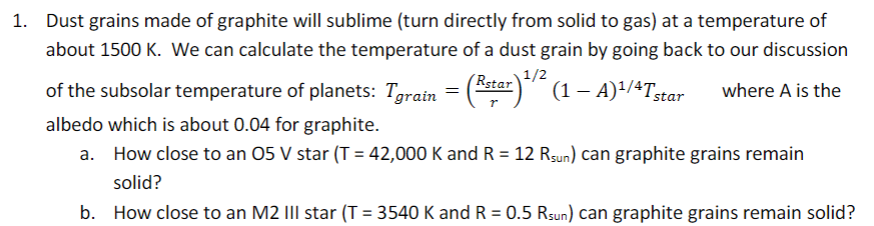
\includegraphics[scale = 0.8]{problemset9prob1.PNG}
\newline
To begin, note that we will want to use the given equation for subsolar temperature to find the distance where a grain of graphite can remain solid. That is, we must solve the above equation for $r$. Doing so, we find
\begin{equation}
    r = \left(\frac{T_{Star}}{T_{Grain}}\right)^2(1-A)^{1/2}R_{Star}
\end{equation}
In our case, since we wish to find the minimum distance to a star such that graphite remains solid, we can use the sublimation temperature for graphite, 1500 $K$.


a) We are given $T_{Star} = 42000 \:K$ and $R_{Star} = 12 \: R_{\odot}$. Plugging these values into (1), we find
\[r_{O} = \left(\frac{42000}{1500}\right)^2 0.96^{1/2}(12 \: R_{\odot})\]
\[\approx 9218 \:R_{\odot}\]
\[\approx 42.87 \:AU\]
So graphite can get as close as approximately $42.87 \:AU$ to an O5 V star with radius $12 \: R_{\bigodot}$ before it sublimates.
\newline

b) We are given $T_{Star} = 3540 \:K$, and $R_{Star} = 0.5 \:R_{\odot}$. Plugging these values into (1), we find
\[r_M = \left(\frac{3540}{1500}\right)^2 0.96^{1/2} (0.5 \:R_{\odot})\]
\[\approx 2.729 \: R_{\odot}\]
\[\approx 0.01269 \:AU\]
So graphite can get as close as approximately 2.729 solar radii to an M2III star with radius $0.5 \: R_{\bigodot}$ before it sublimates.
\newline

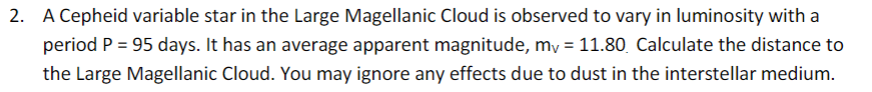
\includegraphics[scale = 0.8]{problemset9prob2.PNG}
\newline

Recall the formula that relates absolute magnitude to the period of a pulsating variable star:
\begin{equation}
    M_v = -2.76\log_{10}{\left(\frac{P}{10 \:\text{days}}\right)} - 4.16
\end{equation}
We are given that the period ($P$) is 95 days, so plugging this value into (2), we find
\[M_v = -2.76 \log_{10}{\left(\frac{95 \:\text{days}}{10 \:\text{days}}\right)} - 4.16\]
\[\approx -6.86\]
So we have that the absolute magnitude of this star is approximately Mag -6.86. Now, we can use the following formula that relates apparent magnitude and absolute magnitude to distance:
\begin{equation}
    M_v = m_v + 5 - 5\log_{10}{(d)}
\end{equation}
where $d$ is in parsecs. Plugging in the given value for $m_v$ and the value we found for $M_v$ into (2) and solving for $d$, we find
\[d = 10^{23.66/5}\]
\[\approx 54000 \: pc\]
\[\approx 17600 \: ly\]
So the Large Magellanic Cloud is approximately $54000 \: pc$ or $17600 \:ly$ away, based on the measurements of this Cepheid variable.
\newline

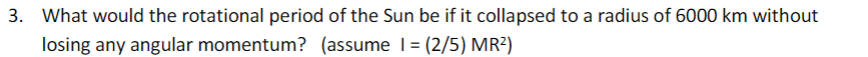
\includegraphics[scale = 0.8]{problemset9prob3.PNG}
\newline

To begin, we first wish to calculate the current moment of inertia of the Sun. That is, its moment of inertia before it suddenly collapses.

First, we note that the mass of the sun is approximately $1.988 \times 10^{30} \: kg$ and the current radius of the Sun is $6.957 \times 10^8 \:m$. Plugging these values into the expression for moment of inertia, we find
\[I_{\odot} = \frac{2}{5}(1.988 \times 10^{30} \:kg)(6.957 \times 10^8 \:m)\]
\[\approx 3.849 \times 10^{47} \:kg\: m^2\]
Now, recall that angular momentum is given by
\begin{equation}
    L_{\odot} = I_{\odot} \omega
\end{equation}
where $\omega$ is the angular velocity of the Sun's rotation. Now we must find $\omega$ for Sun in its current state.
\[\omega = \frac{v}{r}\]
\[= \frac{1.990 \times 10^3 \:m\:s^{-1}}{6.957 \times 10^8 \:m}\]
\[\approx 2.860 \times 10^{-6} \:\text{rad} \: s^{-1}\]
And plugging this into (4), we find
\[L_{\odot} \approx 1.100 \times 10^{42} \:kg\:m^2 s^{-1}\]
Now let's calculate the moment of inertia of the Sun if it had a radius of $6000 \:km$ (assuming the same mass):
\[I'_{\odot} = \frac{2}{5} (1.988 \times 10^{30} \:kg)(6000 \times 10^3 \:m)^2\]
\[\approx 2.863 \times 10^{43} \:kg\:m^2\]
Now, we wish to find $\omega '$. Since angular momentum is assumed to be conserved, we have that
\[L_{\odot} = I'_{\odot} \omega ' = 1.100 \times 10^{42} \:kg\:m^2 s^{-1}\]
Plugging in the value we found for $I'_{\odot}$ into the above equation and solving for $\omega '$, we find
\[\omega ' \approx 0.0384 \:\text{rad}\:s^{-1}\]
And to find how long it takes for the Sun to complete one period of rotation, simply divide $2\pi$ by $\omega '$.

\[P = \frac{2\pi}{0.0384 \:s^{-1}}\]
\[\approx 163.6 \:s\]
That is, if the Sun suddenly collapsed down to a radius of $6000 \:km$, it would rotate about once every 163 seconds. Fewer than three minutes!
\newline


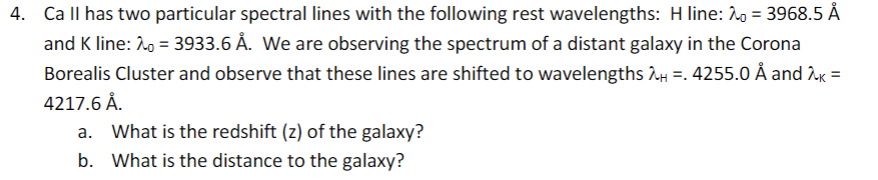
\includegraphics[scale = 0.8]{problemset9prob4.PNG}
\newline

a) Recall that the redshift ($z$) is defined by
\begin{equation} 
z = \frac{\lambda_{\text{observed}} - \lambda_{\text{emitted}}}{\lambda_{\text{emitted}}} 
\end{equation}

From the given values, We have that $\lambda_{\text{emitted}, \text{H}} = 3968.5 \: \text{\AA}$, and $\lambda_{\text{emitted}, \text{K}} = 3933.6 \: \text{\AA}$. 
And for the observed values, we have $\lambda_{\text{observed},\text{H}} = 4255.0 \: \text{\AA}$ and $\lambda_{\text{observed},\text{K}} = 4217.6 \: \text{\AA}$. Using these values and plugging them into (5), we find 
\[z = \frac{\lambda_{\text{observed},\text{H}} - \lambda_{\text{emitted},\text{H}}}{\lambda_{\text{emitted},\text{H}}}\]
\[ = \frac{4255.0 \: \text{\AA} - 3968.5 \: \text{\AA}}{3968.5 \: \text{\AA}}\]
\[\approx 7.2198 \times 10^{-2}\]
and we find the same thing for the K line:
\[z = \frac{\lambda_{\text{observed}, \text{K}} - \lambda_{\text{emitted}, \text{K}}}{\lambda_{\text{emitted}, \text{K}}}\]
\[ = \frac{4217.6 \: \text{\AA} - 3933.6 \: \text{\AA}}{3933.6 \: \text{\AA}}\]
\[\approx 7.2198 \times 10^{-2}\]
So the redshift ($z$) of this galaxy is approximately $7.2198 \times 10^{-2}$ or $0.072198$.
\newline

b) Recall the relationship between $d$ and $z$:
\[d = \frac{cz}{H_0}\]
where $H_0$ is the Hubble constant. Using a value of $70 \: \frac{km}{s \:MPc}$ for $H_0$, we find
\[d = \frac{(3 \times 10^5 \: km/s)(0.072198)}{70 \: km/sMPc}\]
\[\approx 309.42 \:MPc\]
So the distance to this galaxy is approximately $309.42 \:MPc$.





\end{document}
